\documentclass[9pt, a4paper, landscape, twocolumn]{scrartcl}

\usepackage{vorschule}
\usepackage[
    typ=ab,
    fach=Mathematik,
    lerngruppe={Q1 GK},
    nummer=4,
    module={Symbole,Lizenzen},
    seitenzahlen=keine,
    farbig,
    lizenz=cc-by-nc-sa-4,
]{schule}

\usepackage[
	kuerzel={Ngb},
	reihe={Analysis},
	version={2019-06-17},
]{ngbschule}

\author{J. Neugebauer}
\title{Die $e$-Funktion}
\date{\Heute}

\renewcommand{\arraystretch}{1.6}

\begin{document}
    \section*{Exponentialfunktionen}
    \[ f(x) = a\cdot b^x = a\cdot e^{\ln{b}x} \]
    \begin{multicols}{2}
    \begin{description}
        \item[$a$] Startwert
        \item[$e$] $\approx 2,7183$
        \item[$b>1$] Wachstumsfaktor ($\ln{b}>0$)
        \item[$0<b<1$] Abnahmefaktor ($\ln{b}<0$)
    \end{description}
    \end{multicols}
    
    \section*{Eigenschaften der $e$-Funktion}
    Für $f(x)=e^{k\cdot x},\ k \geq 1$ gilt:
    \begin{multicols}{2}
        \begin{tikzpicture}[scale=0.4]
            \geoInit[xmin=-5,xmax=5,ymin=-.5,ymax=5]
            \tkzDrawXY[label={},]
            %\geoGitter
            \tkzFct[color=NavyBlue,line width=1.2]{2.71828 ** \x}
            \geoText(2.3,4.4){$e^x$}
        \end{tikzpicture}
        
        \columnbreak
            
        \begin{itemize}\itemsep 0pt
            \item $f(0)=1$
            \item $f(x)>0$ für alle $x\in \R$
            \item $f$ wächst steng monoton
            \item $f(x)\to \infty$ für $x\to \infty$
            \item $f(x)\to 0$ für $x\to -\infty$
        \end{itemize}
    \end{multicols}
    
    Für $f(x)=e^{k\cdot x},\ k \leq -1$ gilt:
    \begin{multicols}{2}
        \begin{tikzpicture}[scale=0.4]
            \geoInit[xmin=-5,xmax=5,ymin=-.5,ymax=5]
            \tkzDrawXY[label={},]
            %\geoGitter
            \tkzFct[color=NavyBlue,line width=1.2]{2.71828 ** (-1 * \x)}
            \geoText(4.2,.8){$e^{-x}$}
        \end{tikzpicture}
        
        \columnbreak
        
        \begin{itemize}\itemsep 0pt
            \item $f(0)=1$
            \item $f(x)>0$ für alle $x\in \R$
            \item $f$ fällt steng monoton
            \item $f(x)\to 0$ für $x\to \infty$
            \item $f(x)\to -\infty$ für $x\to -\infty$
        \end{itemize}
    \end{multicols}
    
    \section*{Kombinationen der $e$-Funktion}\vspace{-2ex}
    \begin{tabularx}{\columnwidth}{Xc}
    	$f(x) = k\cdot e^x$
    	
    	\begin{itemize}
    		\item $f(0)=k$
    	\end{itemize}\itemsep 0pt
    		&\begin{tikzpicture}[scale=0.4,baseline=(current bounding box.north)]
    		\geoInit[xmin=-4,xmax=4,ymin=-.5,ymax=4]
    		\tkzDrawXY[label={},]
    		\tkzFct[color=NavyBlue,line width=1.2]{2 * 2.71828 ** \x}
    		\geoText(2.3,3.4){$2\cdot e^x$}
    		\end{tikzpicture} \\
    		
    	$f(x) = x^k\cdot e^x$, $k$ gerade 
    	
    	\begin{itemize}\itemsep 0pt
    		\item Hochpunkt bei $x = -k$
    		\item Tiefpunkt bei \pkt(0|0) für $k=2$
    		\item Sattelpunkt bei \pkt(0|0) für $k > 2$
    	\end{itemize}
    		&\begin{tikzpicture}[scale=0.4,baseline=(current bounding box.north)]
    		\geoInit[xmin=-6,xmax=2,ymin=-.5,ymax=4]
    		\tkzDrawXY[label={},]
    		\tkzFct[color=NavyBlue,line width=1.2]{(\x ** 2) * (2.71828 ** \x)}
    		\geoText(-1.5,1.4){$x^2\cdot e^x$}
    		\end{tikzpicture} \\
    		
   		$f(x) = x^k\cdot e^x$, $k$ ungerade 
   		
   		\begin{itemize}\itemsep 0pt
   			\item $f(0) = 0$
   			\item Tiefpunkt bei $x = -k$
   			\item Sattelpunkt bei \pkt(0|0)
   		\end{itemize}
    		&\begin{tikzpicture}[scale=0.4,baseline=(current bounding box.north)]
    		\geoInit[xmin=-6,xmax=2,ymin=-1.5,ymax=4]
    		\tkzDrawXY[label={},]    		
    		\tkzFct[color=NavyBlue,line width=1.2]{(\x ** 3) * (2.71828 ** \x)}
    		\geoText(-1.5,1){$x^3\cdot e^x$}
    		\end{tikzpicture} \\
    		
        $f(x) = k\cdot e^x + k\cdot e^{-x}$
        
        \begin{itemize}\itemsep 0pt
        	\item $f(0) = 2k$
        	\item Tief- ($k>0$)/Hochpunkt ($k<0$) bei \pkt(0|2k)
        	\item Achsensymmetrisch $f(x) = f(-x)$
        \end{itemize}
		    &\begin{tikzpicture}[scale=0.4,baseline=(current bounding box.north)]
			\geoInit[xmin=-2,xmax=2,ymin=0,ymax=6]
			\tkzDrawXY[label={},]    		
			\tkzFct[color=NavyBlue,line width=1.2]{2.71828 ** \x + 2.71828 ** (-1 * \x)}
			\geoText(-2,1){$e^x + e^{-x}$}
			\end{tikzpicture}\\
			
        $f(x) = e^{k\cdot x} - e^{k\cdot -x}$
        
        \begin{itemize}\itemsep 0pt
        	\item $f(0) = 0$
        	\item Punktsymmetrisch $-f(x) = f(-x)$
        	\item Streng monoton wachsend ($k>0$)/fallend ($k<0$)
        \end{itemize}
		    &\begin{tikzpicture}[scale=0.4,baseline=(current bounding box.north)]
			\geoInit[xmin=-3,xmax=3,xstep=1,ymin=-12,ymax=12,ystep=4]
			\tkzDrawXY[label={},]    		
			\tkzFct[color=NavyBlue,line width=1.2]{2.71828 ** \x - 2.71828 ** (-1 * \x)}
			\geoText(-2,3.4){$e^{x} - e^{-x}$}
			\end{tikzpicture} \\
    \end{tabularx}


	\section*{Produkt aus e-Funktion und Polynomen}
	\[ f(x) = g(x)\cdot e^x  \]
	\begin{description}
		\item[$g_n(x)$] Ganzrationale Funktion (Polynom) vom Grad n.
		\item[$h(x)$] e-Funktion ($h(x) = e^{mx+b}$)
	\end{description}

	\begin{itemize}
		\item Ableitung mit Produktregel
		\[ f'(x) = g_n'(x)\cdot h(x) + g_(x)\cdot h'(x) \]
		\item Nullstellen:
		\[ f(x) = 0 \Leftrightarrow g_n(x) = 0,\qquad \text{da }h(x)> 0\text{ für alle } x\]
		\item Verlauf im Unendlichen:
		
		Die $e$-Funktion wächst stärker als jede ganzrationale Funktion! Das Verhalten für $x\to \infty$ bzw, $x\to -\infty$ wird also von $h(x)$ bestimmt:
		
		\begin{itemize}
			\item $f(x)\to \infty \Leftrightarrow h(x)\to \infty$
			\item $f(x)\to -\infty \Leftrightarrow h(x)\to -\infty$
			\item $f(x)\to 0 \Leftrightarrow h(x)\to 0$
		\end{itemize}
	\end{itemize}

	\newpage

	\begin{center}
		\begin{tikzpicture}[scale=0.6]
		\geoInit[xmin=-6,xmax=6,ymin=-24,ymax=24,ystep=3]
		\tkzDrawXY[label={},]
		\tkzFct[color=NavyBlue,line width=1.2,domain=-8:3]{(\x ** 2 - 5) * (2.71828 ** \x)}
		\geoText(4,21){$(x^2-5)\cdot e^{x}$}
		\tkzFct[color=RedViolet,line width=1.2,domain=-1.5:6]{(7 * \x ** 3 + 6 * \x ** 2) * (2.71828 ** (-3*\x))}
		\geoText(-3.5,-15){$(7x^3 + 6x^2)\cdot e^{-3x}$}
		\end{tikzpicture}
	\end{center}
\end{document}